\section{Risk Assessment}
\label{sec:risk-assessment}

As discussed in section \ref{sec:pool-management}, DynaFed leverages collateralization levels and dynamic capacity targets when allocating pegins and assigning pegouts. However, these mechanisms should also influence pool lifecycle management itself. We employ a selection bias favoring reliable, well-functioning pools while disadvantaging under-performers and \textbf{eventually sunsetting problematic pools}. The top priority is fund security, requiring swift action when a pool experiences member attrition or operational degradation.

We apply this bias through a simple sigmoid risk adjustment factor $\phi(r)$ that modulates a pool's effective collateralization. Following a \textit{"first gradually, then suddenly"} approach, we exercise caution when allocating to newly established pools and when determining sunset timing for failing pools. The function $\phi(r)$ produces a value in $[0, 1]$ that scales the nominal collateralization level $C_M$ as defined in section \ref{sec:collateralization-level}, yielding an effective collateralization of $C_M \times \phi(r_M)$. When $\phi(r_M) = 1$, the pool operates at full capacity with complete collateralization leverage. When $\phi(r_M) = 0$, the pool is effectively defunct and must be sunset.

We define the \textbf{risk adjustment factor} as:

\begin{equation}
    \label{eq:risk-sigmoid}
    \phi(r) = \frac{1}{1 + e^{k(r - r_{mid})}}
\end{equation}

and visualized in figure \ref{fig:sigmoid-capacity}, where $k=15$ and $r_{mid}=0.5$. We employ a balanced sigmoid curve without excessive parameter tuning, as the primary complexity lies in computing $r$, the \textbf{risk level} as defined in section \ref{sec:risk-level-calculation}.

\begin{figure}[h]
    \centering
    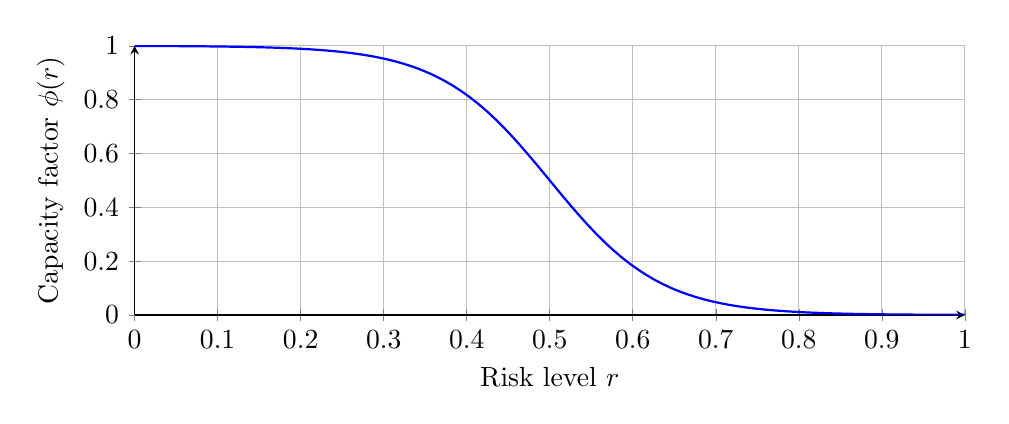
\begin{tikzpicture}
        \begin{axis}[
                width=\columnwidth,
                height=5cm,
                xlabel={Risk level $r$},
                ylabel={Capacity factor $\phi(r)$},
                domain=0:1,
                samples=100,
                grid=major,
                ymin=0, ymax=1,
                xmin=0, xmax=1,
                axis lines=left,
                enlarge x limits=false,
                enlarge y limits=false,
            ]
            \addplot[blue, thick] {1 / (1 + exp(15*(x - 0.5)))};
        \end{axis}
    \end{tikzpicture}
    \caption{\small Sigmoid capacity function $\phi(r)$ modulating effective collateralization based on pool risk level}
    \label{fig:sigmoid-capacity}
\end{figure}

\subsection{Risk Level}
\label{sec:risk-level-calculation}

The risk level $r_M$ quantifies the operational health of pool $M$ by assessing the participation and reliability of its members, with a preference toward established, proven validators. This metric feeds directly into the capacity adjustment function $\phi(r_M)$ defined in equation \ref{eq:risk-sigmoid}, determining the pool's effective collateralization.

DynaFed tracks individual member weights and aggregates them to compute the \textbf{pool-level risk}:

\begin{equation}
    \label{eq:aggr-risk-level}
    r_M = 1 - \frac{\sum_{m \in M} w(m)}{|M|}
\end{equation}

where $w(m)$ is the \textbf{member weight} for member $m$, defined as:

\begin{equation}
    w(m) = \sigma_M \times \psi_M \times \left(\alpha \times s_m + (1-\alpha) \times t_m\right)
\end{equation}

with components:
\begin{itemize}
    \item $\sigma_M \in \{0, 1\}$: state control parameter as defined in section \ref{sec:state-control-parameter}
    \item $\psi_M \in \{0, 1\}$: emergency controller as defined in section \ref{sec:emergency-controller}
    \item $\alpha \in [0.5, 0.7]$: weight parameter balancing recent performance versus long-term tenure
    \item $s_m$: participation score as defined in section \ref{sec:participation-score}
    \item $t_m$: tenure score as defined in section \ref{sec:tenure-score}
\end{itemize}

\subsubsection{State Control Parameter}
\label{sec:state-control-parameter}

The state control parameter $\sigma_M$ acts as an activation gate that prevents premature capacity allocation during the observation window when block samples are insufficient for reliable member scoring. Newly established pools require time to accumulate sufficient data before their participation and tenure scores can meaningfully reflect operational health.

The state control parameter is defined as:

\begin{equation}
    \label{eq:state-control-parameter}
    \sigma_M = \begin{cases}
        0 & \text{if } b - b_0^M < N_{\min} \text{ or } p_M < |M|     \\
        1 & \text{if } b - b_0^M \geq N_{\min} \text{ and } p_M = |M|
    \end{cases}
\end{equation}

where:
\begin{itemize}
    \item $b$: current block height
    \item $b_0^M$: block height when pool $M$ was created (after DKG completion)
    \item $N_{\min}$: minimum observation period (e.g., 100 blocks $\approx$ 10 minutes)
    \item $p_M = |\{m \in M : s_m(b) > 0\}|$: count of members who have submitted at least one FROST proof, where $s_m$ is participation score as described in section \ref{sec:participation-score}.
\end{itemize}

During the observation window ($\sigma_M = 0$), all member weights become zero regardless of their individual participation or tenure scores. This suppresses the influence of high volatility in both $s_m$ and $t_m$ that occurs when few blocks have elapsed. The pool remains in this dormant state until sufficient time has passed to establish reliable scoring patterns.

Once $\sigma_M$ transitions to 1, the pool is considered \textbf{activated} and its risk level directly reflects member performance through the standard risk calculation. Conceptually, a pool is being \textbf{onboarded} when $\sigma_M = 0$ during the observation phase, which forces $r_M = 1$ regardless of individual member scores. A pool is being \textbf{offboarded} or sunset when $\sigma_M = 1$ but $r_M \to 1$ due to member degradation, triggering capacity wind-down through the sigmoid function. This binary state transition ensures a clean separation between the observation phase and normal operational status.

\subsubsection{Emergency Controller}
\label{sec:emergency-controller}

The emergency controller $\psi_M$ provides a critical safety mechanism that forces immediate pool shutdown when the number of active members approaches the FROST signing threshold. While the gradual risk assessment through $\phi(r_M)$ handles normal operational degradation, FROST threshold signatures require a minimum number of functioning members to execute transactions. If a pool degrades to the point where it risks falling below this operational threshold, gradual wind-down is insufficient; the pool must be sunset immediately before it becomes unable to sweep its own funds.

The emergency controller is defined as:

\begin{equation}
    \label{eq:emergency-controller}
    \psi_M = \begin{cases}
        0 & \text{if } A_M < \lceil |M| \times \rho_{\text{safety}} \rceil \\
        1 & \text{otherwise}
    \end{cases}
\end{equation}

where:
\begin{itemize}
    \item $A_M = |\{m \in M : s_m(b) > \theta_{\text{active}}\}|$: count of members exceeding the liveness threshold
    \item $\theta_{\text{active}}$: liveness threshold for considering a member "active" (e.g., 0.8)
    \item $\rho_{\text{safety}} = \frac{t_M}{|M|} + \epsilon_M$: safety ratio relative to FROST threshold
    \item $t_M$: FROST signing threshold for pool $M$ (e.g., 12 for a 12-of-16 multisig)
    \item $\epsilon_M$: collateralization-aware safety buffer
\end{itemize}

The safety buffer $\epsilon_M$ adapts based on pool tier and collateralization status:

\begin{equation}
    \label{eq:safety-buffer}
    \epsilon_M = \begin{cases}
        \epsilon_{\text{strict}} & \text{if Tier 1 or } F_M > C_M     \\
        0                        & \text{if Tier 2 and } F_M \leq C_M
    \end{cases}
\end{equation}

where $\epsilon_{\text{strict}} = 0.125$ provides a safety buffer above the FROST threshold as a fraction of pool size, and $F_M$ and $C_M$ are the pool's current funds and total collateralization as defined in section \ref{sec:collateralization-level}.

\textbf{Design Rationale}: Tier 1 pools and under-collateralized Tier 2 pools maintain strict safety buffers because fund loss is possible if the pool becomes inoperable. Over-collateralized Tier 2 pools use $\epsilon_M = 0$, triggering emergency shutdown only at the actual FROST threshold. This relaxed approach is justified because these pools have full collateral backing on Tier 1. The worst-case failure is service degradation (pegout delays), not fund loss. This provides maximum operational flexibility for hot wallets while the collateral guarantee provides the safety net.

When $\psi_M = 0$, all member weights become zero regardless of individual scores, forcing $r_M = 1$ and consequently $\phi(r_M) \approx 0$. This immediately halts new pegin allocation to the pool and triggers urgent fund sweeping to healthy pools.

\subsubsection{Participation Score}
\label{sec:participation-score}

The participation score $s_m$ measures the recent liveness and responsiveness of member $m$. Members prove their active participation by submitting FROST signature proofs via the NDD as described in section \ref{sec:foundation-layer}. These proofs serve dual purposes: they demonstrate that members possess their key material and are online, actively participating in consensus.

A critical constraint is that FROST proof submission requires the member to be selected as block producer, enabling them to include their proof in the NDD. This means members compete for block production slots not just among pool members $|M|$, but across the entire validator set $N_v$. We assume CometBFT's fair block producer selection guarantees that over sufficient time, every validator has approximately equal opportunity to produce blocks. Members may implement external gossiping mechanisms allowing others to include their proofs on their behalf, which is secure given that FROST proofs are cryptographically signed.

The participation score uses an exponentially weighted moving average (EWMA), similar to the dynamic capacity target in section \ref{sec:dynamic-capacity-target}. This approach is computationally efficient, requires minimal storage, and naturally adapts to changing behavior:

\begin{equation}
    \label{eq:participation-score}
    s_m(b) = \beta \times p_m(b) \times N_v + (1 - \beta) \times s_m(b-1)
\end{equation}

where:
\begin{itemize}
    \item $s_m(b)$: participation score at block height $b$
    \item $p_m(b) \in \{0, 1\}$: proof indicator (1 if member $m$ submitted valid FROST proof in block $b$, 0 otherwise)
    \item $N_v$: total number of validators in the network
    \item $\beta \in [0.001, 0.01]$: smoothing factor controlling responsiveness versus stability
\end{itemize}

The $N_v$ scaling factor normalizes for expected block production frequency, ensuring that members who consistently submit proofs when selected converge to $s_m \approx 1$, while unreliable members decay toward $s_m \approx 0$. The initial condition is $s_m(b_0^M) = 0$, requiring new members to establish their reliability through observed behavior.

The smoothing factor $\beta$ is intentionally small because the EWMA updates every block (every 6 seconds), while individual members produce blocks infrequently at rate $1/N_v$. This ensures the score smooths over multiple block production opportunities rather than reacting to single events.

\subsubsection{Tenure Score}
\label{sec:tenure-score}

The tenure score $t_m$ measures how long a member has been part of an active pool, reflecting establishment and stability within the system. Unlike the participation score which tracks recent performance, tenure captures long-term presence independent of current behavior. This distinction ensures that newly activated members with perfect participation still operate at reduced weight until they prove sustained reliability over time.

Tenure is calculated as the fraction of time elapsed since pool activation, capped at the maturity threshold:

\begin{equation}
    t_m = \min\left(1, \frac{b - b_0^M}{N_{\text{maturity}}}\right)
\end{equation}

where:
\begin{itemize}
    \item $t_m$: tenure score for member $m$
    \item $b$: current block height
    \item $b_0^M$: block height when pool $M$ was activated
    \item $N_{\text{maturity}}$: maturity threshold (e.g., 14,400 blocks $\approx$ 24 hours)
\end{itemize}

All members of pool $M$ share the same tenure score since it depends only on pool activation time, not individual member behavior. A newly activated pool begins with $t_m = 0$ for all members, reaching full tenure credit ($t_m = 1$) after $N_{\text{maturity}}$ blocks of operation. This creates the "gradually, then suddenly" capacity ramp described in section \ref{sec:risk-assessment}, where new pools start with limited effective collateralization that grows as they demonstrate sustained operational stability.

The tenure score is computationally trivial, requiring only two block height values and basic arithmetic, and provides the timespan that complements the performance-based participation score in the composite member weight.
